%!TEX encoding = UTF-8 Unicode
\documentclass[french, a4paper, 12pt, twocolumn, landscape]{article}



%% Langue et compilation

\usepackage[utf8]{inputenc}
\usepackage[T1]{fontenc}
\usepackage[french]{babel}

%% LISTE DES PACKAGES

\usepackage{mathtools}     % package de base pour les maths
\usepackage{amsmath}       % mathematical type-setting
\usepackage{amssymb}       % symbols speciaux pour les maths
\usepackage{textcomp}      % symboles speciaux pour el text
\usepackage{gensymb}       % commandes generiques \degree etc...
\usepackage{tikz}          % package graphique
\usepackage{wrapfig}       % pour entourer a cote d'une figure
\usepackage{color}         % package des couleurs
\usepackage{xcolor}        % autre package pour les couleurs
\usepackage{pgfplots}      % pacakge pour creer des graph
\usepackage{epsfig}        % permet d'inclure des graph en .eps
\usepackage{graphicx}      % arguments dans includegraphics
\usepackage{pdfpages}      % permet d'insérer des pages pdf dans le document
\usepackage{subfig}        % permet de creer des sous-figure
\usepackage{pst-all}       % utile pour certaines figures en pstricks
\usepackage{lipsum}        % package qui permet de faire des essais
\usepackage{array}         % permet de faire des tableaux
\usepackage{multicol}      % plusieurs colonnes sur une page
\usepackage{enumitem}      % pro­vides user con­trol: enumerate, itemize and description
\usepackage{hyperref}      % permet de creer des hyperliens dans le document
\usepackage{lscape}        % permet de mettre une page en mode paysage
\usepackage{lmodern}       % permet d'avoir certains "fonts" de bonen qualite
\usepackage{fancyhdr}      % Permet de mettre des informations en hau et en bas de page      
\usepackage[framemethod=tikz]{mdframed} % breakable frames and coloured boxes
\usepackage[top=1.5cm, bottom=1.5cm, left=2.5cm, right=2.5cm]{geometry} % donne les marges
\usepackage[font=normalsize, labelfont=bf,labelsep=endash, figurename=Fig.]{caption} % permet de changer les legendes des figures
\usepackage{lewis}
\usepackage{bohr}
\usepackage{chemfig}
\usepackage{chemist}

%% LIBRAIRIES

\usetikzlibrary{plotmarks} % librairie pour les graphes
\usetikzlibrary{patterns}  % necessaire pour certaines choses predefinies sur tikz
\usetikzlibrary{shadows}   % ombres des encadres
\usetikzlibrary{backgrounds} % arriere plan des encadres


%% MISE EN PAGE

\pagestyle{fancy}     % Défini le style de la page

\renewcommand{\headrulewidth}{1pt}      % largeur du trait en haut de la page
\fancyhead[L]{Seconde générale}         % info coin haut gauche
\fancyhead[R]{Lycée Jean Guéhenno}  % info coin haut droit

% bas de la page
\renewcommand{\footrulewidth}{1pt}      % largeur du trait en bas de la page
\fancyfoot[L]{G. \bsc{LE DOUDIC}}  % info coin bas gauche
\fancyfoot[R]{TP 4 : Famille chimique}                         % info coin bas droit


\setlength{\columnseprule}{1pt} 
\setlength{\columnsep}{30pt}



%% NOUVELLES COMMANDES 

\DeclareMathOperator{\e}{e} % permet d'ecrire l'exponentielle usuellement


\newcommand{\gap}{\vspace{0.15cm}}   % defini une commande pour sauter des lignes
\renewcommand{\vec}{\overrightarrow} % permet d'avoir une fleche qui recouvre tout le vecteur
\newcommand{\bi}{\begin{itemize}}    % begin itemize
\newcommand{\ei}{\end{itemize}}      % end itemize
\newcommand{\bc}{\begin{center}}     % begin center
\newcommand{\ec}{\end{center}}       % end center
\newcommand\opacity{1}               % opacity 
\pgfsetfillopacity{\opacity}

\newcommand*\Laplace{\mathop{}\!\mathbin\bigtriangleup} % symbole de Laplace

\frenchbsetup{StandardItemLabels=true} % je ne sais plus

\newcommand{\smallO}[1]{\ensuremath{\mathop{}\mathopen{}o\mathopen{}\left(#1\right)}} % petit o

\newcommand{\cit}{\color{blue}\cite} % permet d'avoir les citations de couleur bleues
\newcommand{\bib}{\color{black}\bibitem} % paragraphe biblio en noir et blanc
\newcommand{\bthebiblio}{\color{black} \begin{thebibliography}} % idem necessaire sinon bug a cause de la couleur
\newcommand{\ethebiblio}{\color{black} \end{thebibliography}}   % idem
%%% TIKZ


%% COULEURS 


\definecolor{definitionf}{RGB}{220,252,220}
\definecolor{definitionl}{RGB}{39,123,69}
\definecolor{definitiono}{RGB}{72,148,101}

\definecolor{propositionf}{RGB}{255,216,218}
\definecolor{propositionl}{RGB}{38,38,38}
\definecolor{propositiono}{RGB}{109,109,109}

\definecolor{theof}{RGB}{255,216,218}
\definecolor{theol}{RGB}{160,0,4}
\definecolor{theoo}{RGB}{221,65,100}

\definecolor{avertl}{RGB}{163,92,0}
\definecolor{averto}{RGB}{255,144,0}

\definecolor{histf}{RGB}{241,238,193}

\definecolor{metf}{RGB}{220,230,240}
\definecolor{metl}{RGB}{56,110,165}
\definecolor{meto}{RGB}{109,109,109}


\definecolor{remf}{RGB}{230,240,250}
\definecolor{remo}{RGB}{150,150,150}

\definecolor{exef}{RGB}{240,240,240}

\definecolor{protf}{RGB}{247,228,255}
\definecolor{protl}{RGB}{105,0,203}
\definecolor{proto}{RGB}{174,88,255}

\definecolor{grid}{RGB}{180,180,180}

\definecolor{titref}{RGB}{230,230,230}

\definecolor{vert}{RGB}{23,200,23}

\definecolor{violet}{RGB}{180,0,200}

\definecolor{copper}{RGB}{217, 144, 88}

%% Couleur des ref

\hypersetup{
	colorlinks=true,
	linkcolor=black,
	citecolor=blue,
	urlcolor=black
		   }

%% CADRES


% %%%%%%%%%% DEFINITION
% \newmdenv[tikzsetting={fill=definitionf}, linewidth=2pt, linecolor=definitionl, outerlinewidth=0pt, innertopmargin=5pt, innerbottommargin=5pt, innerleftmargin=5pt, innerrightmargin=5pt, leftmargin=0pt]{definition}

% \newmdenv[ tikzsetting={drop shadow={ shadow xshift=1ex, shadow yshift=-0.5em, fill=definitiono, opacity=1, every shadow } }, outerlinewidth=2pt, outerlinecolor=white, linecolor=white, innertopmargin=0pt, innerbottommargin=0pt, innerleftmargin=0pt, innerrightmargin=0pt]{ombredef}


% %%%%%%%%%% THEOREME

% \newmdenv[tikzsetting={fill=theof}, linewidth=2pt, linecolor=theol, outerlinewidth=0pt, innertopmargin=5pt, innerbottommargin=5pt, innerleftmargin=5pt, innerrightmargin=5pt, leftmargin=0pt]{theo}

% \newmdenv[ tikzsetting={drop shadow={ shadow xshift=1ex, shadow yshift=-0.5em, fill=theoo, opacity=1, every shadow } }, outerlinewidth=2pt, outerlinecolor=white, linecolor=white, innertopmargin=0pt, innerbottommargin=0pt, innerleftmargin=0pt, innerrightmargin=0pt]{ombretheo}


% %%%%%%%%%% METHODE

% \newmdenv[tikzsetting={fill=metf}, linewidth=2pt, linecolor=metl, outerlinewidth=0pt, innertopmargin=5pt, innerbottommargin=5pt, innerleftmargin=5pt, innerrightmargin=5pt, leftmargin=0pt]{met}

% \newmdenv[ tikzsetting={drop shadow={ shadow xshift=1ex, shadow yshift=-0.5em, fill=meto, opacity=1, every shadow } }, outerlinewidth=2pt, outerlinecolor=white, linecolor=white, innertopmargin=0pt, innerbottommargin=0pt, innerleftmargin=0pt, innerrightmargin=0pt]{ombremet}



%%%%%%%%%%% RQ

\newmdenv[tikzsetting={fill=remf}, linewidth=2pt, linecolor=remf, outerlinewidth=0pt, innertopmargin=5pt, innerbottommargin=5pt, innerleftmargin=5pt, innerrightmargin=5pt, leftmargin=0pt]{remarque}

\newmdenv[ tikzsetting={drop shadow={ shadow xshift=1ex, shadow yshift=-0.5em, fill=remo, opacity=1, every shadow } }, outerlinewidth=2pt, outerlinecolor=white, linecolor=white, innertopmargin=0pt, innerbottommargin=0pt, innerleftmargin=0pt, innerrightmargin=0pt]{ombreremarque}

%%%%%%%%%%% Cadre pour le titre

\tikzset{every shadow/.style={opacity=1}}

\global\mdfdefinestyle{doc}{backgroundcolor=white, shadow=true, shadowcolor=propositiono, linewidth=1pt, linecolor=black, shadowsize=5pt}
\global\mdfdefinestyle{titr}{backgroundcolor=metf, shadow=true, shadowcolor=propositiono, linewidth=1pt, linecolor=black, shadowsize=5pt}
\global\mdfdefinestyle{theo}{backgroundcolor=theof, shadow=true, shadowcolor=theoo, linewidth=1pt, linecolor=theol, shadowsize=5pt}
\global\mdfdefinestyle{prop}{backgroundcolor=theof, shadow=true, shadowcolor=propositiono, linewidth=1pt, linecolor=theol, shadowsize=5pt}
\global\mdfdefinestyle{def}{backgroundcolor=definitionf, shadow=true, shadowcolor=definitiono, linewidth=1pt, linecolor=definitionl, shadowsize=5pt}
\global\mdfdefinestyle{histo}{backgroundcolor=histf, shadow=true, shadowcolor=propositiono, linewidth=1pt, linecolor=black, shadowsize=5pt}
\global\mdfdefinestyle{avert}{backgroundcolor=white, shadow=true, shadowcolor=averto, linewidth=1pt, linecolor=avertl, shadowsize=5pt}
\global\mdfdefinestyle{met}{backgroundcolor=metf, shadow=true, shadowcolor=meto, linewidth=1pt, linecolor=metl, shadowsize=5pt}
\global\mdfdefinestyle{rem}{backgroundcolor=metf, shadow=true, shadowcolor=meto, linewidth=1pt, linecolor=metf, shadowsize=5pt}
\global\mdfdefinestyle{exo}{backgroundcolor=exef, shadow=true, shadowcolor=propositiono, linewidth=1pt, linecolor=exef, shadowsize=5pt}
\global\mdfdefinestyle{not}{backgroundcolor=definitionf, shadow=true, shadowcolor=propositiono, linewidth=1pt, linecolor=black, shadowsize=5pt}
\global\mdfdefinestyle{proto}{backgroundcolor=protf, shadow=true, shadowcolor=proto, linewidth=1pt, linecolor=protl, shadowsize=5pt}

%%%%%%
\definecolor{cobalt}{rgb}{0.0, 0.28, 0.67}
\definecolor{applegreen}{rgb}{0.55, 0.71, 0.0}

\usepackage{tcolorbox}
  \tcbuselibrary{most}
  \tcbset{colback=cobalt!5!white,colframe=cobalt!75!black}



\newtcolorbox{definition}[1]{
	colback=applegreen!5!white,
  	colframe=applegreen!65!black,
	fonttitle=\bfseries,
  	title={#1}}
\newtcolorbox{Programme}[1]{
	colback=cobalt!5!white,
  	colframe=cobalt!65!black,
	fonttitle=\bfseries,
  	title={#1}}  

\newtcolorbox{Exercice}[1]{
  colback=cobalt!5!white,
  colframe=cobalt!65!black,
  fonttitle=\bfseries,
  title={#1}}  

  \newtcolorbox{Protocol}[1]{
  colback=cyan!5!white,
  colframe=cyan!65!black,
  fonttitle=\bfseries,
  title={#1}}  

\newtcolorbox{Resultat}[1]{
	colback=theof,%!5!white,
	colframe=theoo!85!black,
  fonttitle=\bfseries,
	title={#1}} 	


\def\width{12}
\def\hauteur{5}

\setlength{\parskip}{0pt}%
\setlength{\parindent}{18pt}


%% MODIFICATION DE CHAPTER  
\makeatletter
\def\@makechapterhead#1{%
  %%%%\vspace*{50\p@}% %%% removed!
  {\parindent \z@ \raggedright \normalfont
    \ifnum \c@secnumdepth >\m@ne
        \huge\bfseries \@chapapp\space \thechapter
        \par\nobreak
        \vskip 20\p@
    \fi
    \interlinepenalty\@M
    \Huge \bfseries #1\par\nobreak
    \vskip 40\p@
  }}
\def\@makeschapterhead#1{%
  %%%%%\vspace*{50\p@}% %%% removed!
  {\parindent \z@ \raggedright
    \normalfont
    \interlinepenalty\@M
    \Huge \bfseries  #1\par\nobreak
    \vskip 40\p@
  }}
  
  \newcommand{\isotope}[3]{%
     \settowidth\@tempdimb{\ensuremath{\scriptstyle#1}}%
     \settowidth\@tempdimc{\ensuremath{\scriptstyle#2}}%
     \ifnum\@tempdimb>\@tempdimc%
         \setlength{\@tempdima}{\@tempdimb}%
     \else%
         \setlength{\@tempdima}{\@tempdimc}%
     \fi%
    \begingroup%
    \ensuremath{^{\makebox[\@tempdima][r]{\ensuremath{\scriptstyle#1}}}_{\makebox[\@tempdima][r]{\ensuremath{\scriptstyle#2}}}\text{#3}}%
    \endgroup%
  }%

\makeatother

\usepackage{eurosym}
\usepackage{colortbl}
% \onehalfspacing
%%
%% DEBUT DU DOCUMENT
%%
\begin{document}


%%%%%%

\titre{Chapitre 11 : Les forces et le principe d'inertie}

\doc{1}{Bulletin officiel}{
\begin{center}
	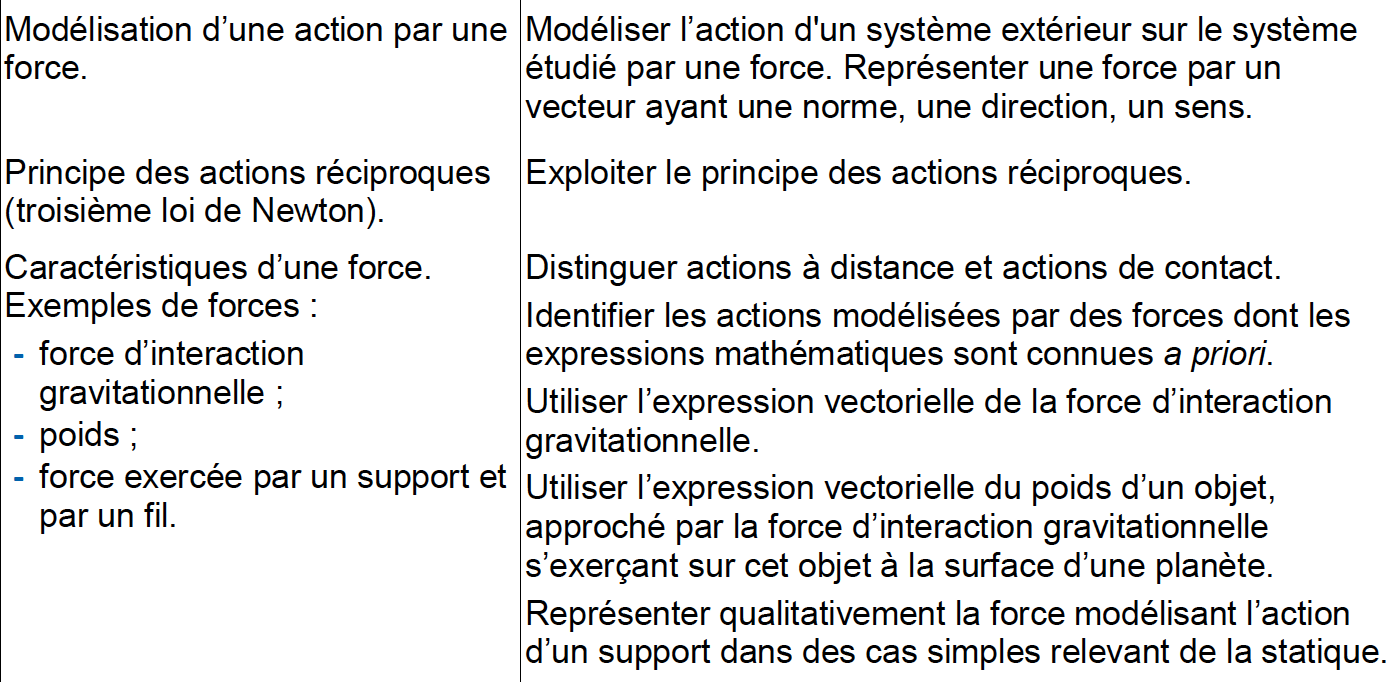
\includegraphics[width=.95\linewidth]{BO1.png}
	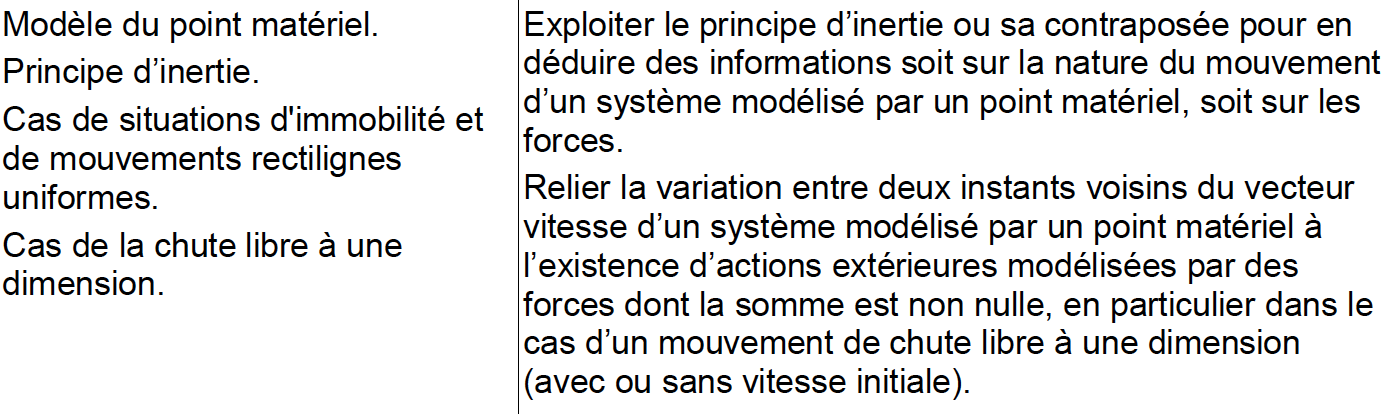
\includegraphics[width=.95\linewidth]{BO2.png}
\end{center}
}


\doc{2}{Exercices dans le livre scolaire}{
		\begin{enumerate}
			\item Actions et forces : exercices 6, 15 et 16 pages 227-228;
			\item Bilan des forces  : exercices 7, 9, 10, 13, 14, et 17 pages 227-228;
			\item Principe d'inertie : exercices 5, 6, 11, 13 et 22 pages 242-243.
		\end{enumerate}
}\vspace{1cm}
	\noindent \textbf{Quiz sur les forces et principe d'inertie}
\begin{center}
	\begin{minipage}{.12\textwidth}
		\centering
		
\includegraphics[width=.5\textwidth]{Quiz1.png}
		
		Quiz 1 - Les actions et forces : \url{https://forms.office.com/r/4hdbcEFLBv?origin=lprLink}
	\end{minipage}\hspace{.5cm}
	\begin{minipage}{.12\textwidth}
		\centering
		
\includegraphics[width=.5\textwidth]{Quiz2.png}

		Quiz 2 - Bilan des forces: \url{https://forms.office.com/r/6AtyTFtMWv?origin=lprLink}
	\end{minipage}\hspace{.5cm}
\begin{minipage}{.12\textwidth}
			\centering
			
\includegraphics[width=.5\textwidth]{Quiz3.png}
	
			Quiz 3 - Le principe d'inertie: \url{https://forms.office.com/r/ChjQWVmWCT?origin=lprLink}
		\end{minipage}
\end{center}

\section*{Introduction}


La Terre exerce une action mécanique sur la Lune, c'est ce qui explique que la Lune orbite autour de la Terre à la manière d'une fronde mise en rotation par un humain. Dans ce chapitre nous allons nous intéresser à comment peut-on modéliser les actions qu'exerce un système extérieur sur un objet. 


\section{Actions mécaniques et forces} 

\begin{center}
	\textit{ref : le livre scolaire page 223}
\end{center}

\subsection{La force, un modèle de l'action d'un système extérieur sur un objet}

Un corps A exerce une action mécanique sur un corps B s'il est capable de provoquer ou de modifier un mouvement du corps B ou encore de le déformer. On modélise ces actions par une force.

\begin{definition}{Définition 1 - Force}
	Une action exercée par un système extérieur sur le système étudié est modélisé par une force notée $\overrightarrow{F}_{A/B}$. Cette force est caractérisée par : 

	\begin{itemize}
		\item une \textbf{norme} notée $F_{A/B} = ||\overrightarrow{F}_{A/B}||$. Il s'agit de la \textbf{valeur} ou de la \textbf{norme} de la force. La valeur de la force s'exprime en newton (N);
		\item une \textbf{direction};
		\item un $\textbf{sens}$.
	\end{itemize}
\end{definition}

\begin{definition}{Définition 2 - Le point matériel}
	En mécanique du point, le système étudié est modélisé par un unique point correspondant au centre de masse du système, c'est le modèle du point matériel.
\end{definition}


\begin{figure}[!ht]
\centering
\begin{tikzpicture}[scale = 1.5]
	\draw[ultra thick] (0,0) node{+};
	% \draw[ultra thick] (1,1) node{+};

	\draw[dashed, thick] (-.5,-.5) -- (1.5,1.5);
	\draw[ultra thick, red, -latex] (0,0) -- (0.8,0.8);
	\draw[ultra thick, red] (2,0.1) node{$\overrightarrow{F}_{\rm~système~extérieur/Système~étudié}$};
\end{tikzpicture}
\end{figure}
\exo{1}{Modéliser le système Terre - ISS}{\realiser On souhaite étudier le mouvement de la station spatiale internationale autour de la Terre. Proposez une modélisation pour étudier le système en mécanique du point.\vspace{2cm}}


\subsection{Deux types de forces}

\begin{Proposition}{Proposition 1 - Deux types de force}
	On classe les actions en deux catégories: 

	\begin{itemize}
		\item \textbf{Les actions de contact};
		\item \textbf{Les actions à distance}.
	\end{itemize}
\end{Proposition}

\exo{2}{Différents types d'actions}{\mobiliser Donner un exemple d'action à distance et un exemple d'action de contact.\vspace{.5cm}}

\subsection{Les diagrammes système-action}
\vspace{-.2cm}
Un diagramme système action permet d'inventorier les actions entre le système étudié et les systèmes extérieurs. 

\exo{3}{Dessiner un diagramme système-action}{
	\realiser Compléter le diagramme système action pour la motocross.

\begin{minipage}{.35\linewidth}
	\centering
	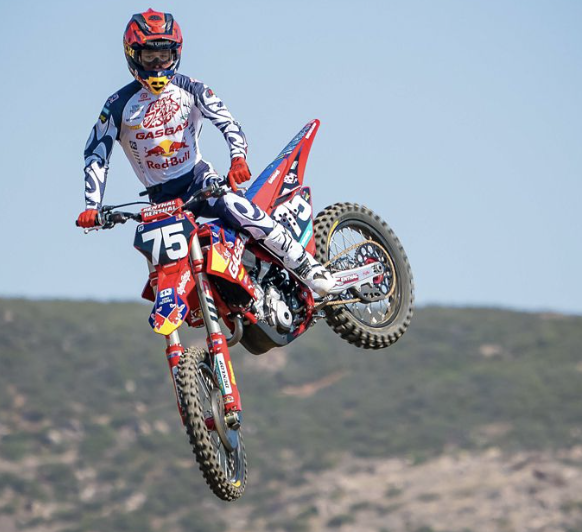
\includegraphics[width=\linewidth]{Motocross.png}
\end{minipage}\hfill
\begin{minipage}{.6\linewidth}
	\centering

	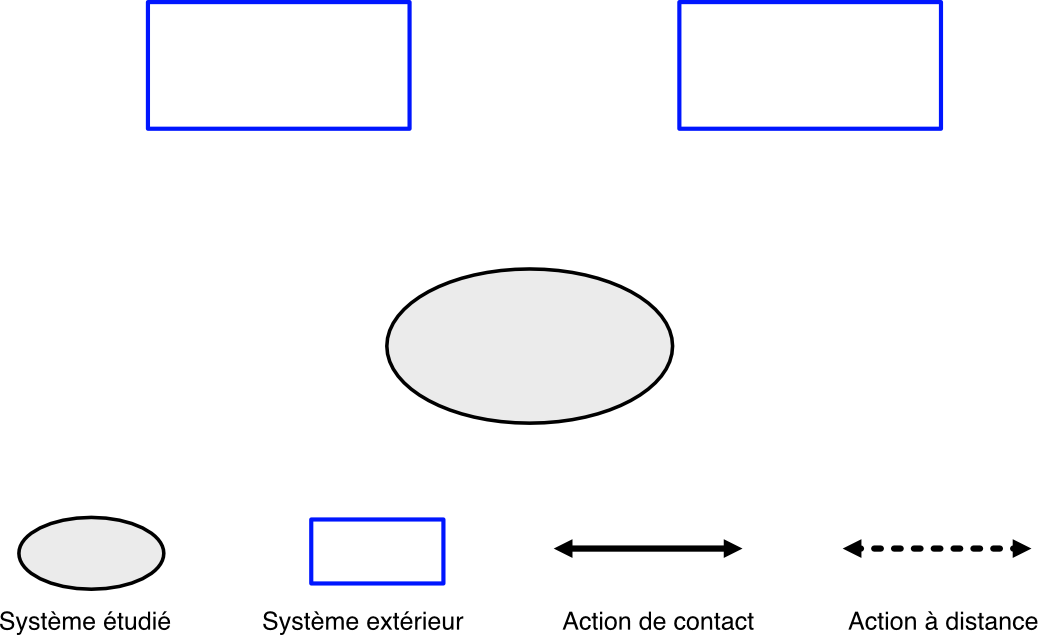
\includegraphics[width=\linewidth]{DiagrameSA_NonComplet.png}
\end{minipage}
}

\section{Le principe des actions réciproques}
\begin{center}
	\textit{ref : le livre scolaire page 223}
\end{center}
\begin{minipage}{.6\linewidth}
	
En 1687, le physicien Isaac Newton énonce le principe des actions réciproques entre deux systèmes, aussi appelé \textbf{$3^{\rm ème}$ loi de Newton} : \medskip

\begin{Proposition}{Principe des actions réciproques - $3^{\rm ème}$ loi de Newton:}
	Lorsqu'un corps A exerce sur un corps B une force $\overrightarrow{F}_{A/B}$ alors B exerce sur A une force $\overrightarrow{F}_{B/A}$ telle que : 

	% $$\vec{F}_{B/A} = -\vec{F}_{A/B}$$
\end{Proposition}
\end{minipage}\hfill
\begin{minipage}{.35\linewidth}
	\histo{Isaac Newton}{
		
		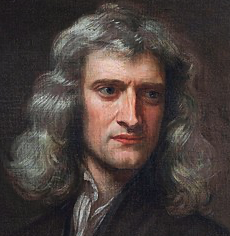
\includegraphics[width=\linewidth]{Newton.png}

		\small{(1642-1727), Il fonde la mécanique classique pour sa théorie de la gravitation universelle.}
	}
\end{minipage}\bigskip

Le principe des actions réciproques s'applique pour des actions de contact ou à distance, que les systèmes soient immobiles ou en mouvement dans le référentiel d'étude.

\exo{4}{Principe des actions réciproques}{\realiser Dessiner les vecteurs des actions de contact et à distance: 

\begin{minipage}{.45\linewidth}
	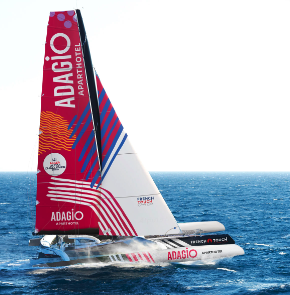
\includegraphics[width=.8\linewidth]{ArkeaEricPeron.png}
\end{minipage}\hfill
\begin{minipage}{.45\linewidth}
	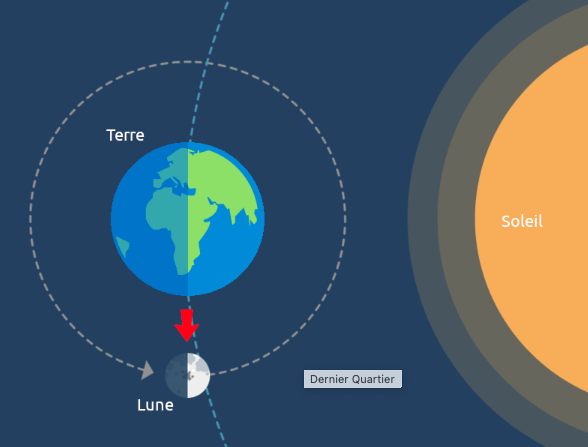
\includegraphics[width=1\linewidth]{TerreSoleilLune.png}
\end{minipage}
}

\section{Exemples de forces caractéristiques}

\begin{center}
	\textit{ref : le livre scolaire page 223}
\end{center}

\subsection{Les caractéristiques du poids}

\begin{definition}{Définition 3 - Le poids $\overrightarrow{P}$}
	Au point de l'espace où se trouve le corps, le poids peut être modélisé par un vecter $\overrightarrow{P}$ ayant pour caractéristiques : 

	\begin{itemize}
		\item  une \textbf{norme} notée $P = ||\overrightarrow{P}|| = m\times g$ et s'exprime en newton (N). La masse $m$ du corps s'exprime en kilogrammes (kg) et $g$ est l'intensité de la pesanteur en $N\cdot kg^{-1}$.
		\item une \textbf{direction} : verticale du lieu considéré
		\item  un $\textbf{sens}$ : du haut vers le bas.
	\end{itemize}
\end{definition}
\subsection{La force exercée par un support}

\begin{definition}{Définition 4 - La réaction du support $\overrightarrow{R}$}
	\medskip
	Dans le cas d'un corps \textbf{immobile} sur lequel ne s'exerce que le poids et la force exercée par le support, la force $\overrightarrow{R}$ compense exactement le poids de ce corps : $$\overrightarrow{R} = - \overrightarrow{P}$$\medskip

	\begin{center}
	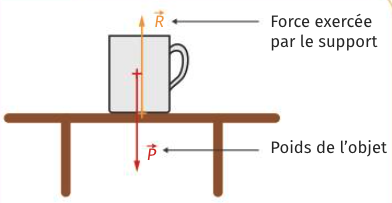
\includegraphics[width=.5\linewidth]{ForceExerceeSupprot.png}
	\end{center}
	%
\end{definition}

\clearpage
\subsection{La force d'interaction gravitationnelle}

\begin{definition}{Définition 5 - Force d'interaction gravitationnelle $\overrightarrow{F}_{A/B}$}

	Au point de l'espace où se trouve un corps B, on modélise l'attraction exercée par un corps A sur ce corps B par un vecteur $\overrightarrow{F}_{A/B}$ ayant pour caractéristiques :

	\begin{itemize}
		\item une \textbf{norme} notée $F_{A/B} = ||\overrightarrow{F}_{A/B}|| = \mathcal{G}\times \dfrac{m_A m_B}{d^2}$ et s'exprime en newton (N). Les masse $m_A$ et $m_B$ des corps s'expriment en kilogrammes (kg) et $d$ la distance séparant A et B en mètres (m) et $\mathcal{G}$ est la \textbf{constante universelle de gravitation}, ayant pour valeur $\mathcal{G}=6,67\times 10^{-11}~\rm N\cdot m^2\cdot kg^{-2}$;\medskip
		\item une \textbf{direction} : droite passant par les centres des corps A et B;\medskip
		\item  un $\textbf{sens}$ : de B vers A (car il s'agit d'une force attractive).
	\end{itemize}
\end{definition}

\exo{5}{Quel est le lien entre $g$ et $\mathcal{G}$}{\realiser Comparer la valeur de $g = 9,81\rm N\cdot kg^{-1}$ à $\mathcal{G}\times \dfrac{M_{Terre}}{R_{Terre}^2}$, sachant que $\mathcal{G} =6,67\times 10^{-11}~\rm N\cdot m^2\cdot kg^{-2}$ $M_{Terre} = 5,972\times 10^{24}~\rm kg$ et $R_{Terre} = 6371~\rm km$.\bigskip

\textbf{Solution:} $\mathcal{G}\times \dfrac{M_{Terre}}{R_{Terre}^2} = 9.81~\rm N\cdot kg^{-1}$. À la surface de la Terre, la force d'attraction gravitationnelle exercée par la Terre et le poids de ce corps sont deux forces égales.

}
\vspace{2cm}
\section{Le principe d'inertie et sa contraposée}

\begin{center}
	\textit{ref : le livre scolaire page 238}
\end{center}

\subsection{Qu'est-il nécessaire de préciser avant toute étude en mécanique ?}
\begin{itemize}
	\item \textbf{Le système étudié} : Quelles que soient la taille, la forme de l'objet d'étude, celui-ci sera modélisé par un point matériel par souci de \textbf{simplification}.\bigskip
	
	\item \textbf{Le référentiel d'étude} : La plupart des études de trajectoires sur Terre se font dans un référentiel terrestre, c'est à dire par rapport à un point lié au sol.
\end{itemize}

\subsection{L'énoncé du principe d'inertie}

En s'appuyant sur les travaux de plusieurs physiciens et mathématiciens, dont ceux ceux de \bsc{Galilée} et \bsc{Descartes}, \bsc{Newton} publie en 1867 \textit{Principia Mathematica}, un ouvrage dans lequel il énonce le principe d'inertie, appelé aussi parfois la \og \textbf{première loi de Newton} \fg

\begin{Proposition}{Principe d'inertie - Première loi de Newton}
	\medskip

	Si les forces qui s'exercent sur un système se compensent, ce système est soit immobile soit en mouvement rectiligne uniforme.
\end{Proposition}

\textbf{Remarque : } La réciproque est vraie : si le système est soit immobile soit en mouvement rectiligne uniforme, alors les forces qui s'exercent sur lui se compensent. 
\subsection{Quel est l'énoncé de la contraposée du principe d'inertie}

\begin{Proposition}{Principe d'inertie - Contraposée de la première loi de Newton}
	\medskip

	Si un système n'est ni immobile ni en mouvement rectiligne uniforme, alors les forces qui s'exercent sur lui ne se compensent pas.\medskip 
\end{Proposition}

\textbf{Remarque:} La réciproque est également vraie.

\exo{6}{Le simulateur de chute libre}{Le simulateur permet de maintenir une personne en l'air grâce à un flux d'air provenant du sol.  On souhaite déterminer la force de poussée de l'air nécessaire pour maintenir immobile une personne ayant une masse $m=65~\rm kg$.

\begin{itemize}
	\item \realiser Faire un schéma de la situation. 

	\begin{tikzpicture}
		\draw[gray, thick, -latex] (1,0) -- (1,-.5) node[left]{$\overrightarrow{g}$};
		\draw[red, thick, -latex] (0,0) -- (0,-1) node[left]{$\overrightarrow{P}$};
		\draw[blue, thick, -latex] (0,0) -- (0,1) node[left]{$\overrightarrow{F}$};
		\draw[thick]  (0,0) node{+};
		\draw[thick] (-.5,0) node{$m$};
	\end{tikzpicture}

	\item \realiser Faire un bilan des forces appliqué à la personne en chute libre. 
	\begin{itemize}
		\item Le poids  (\(\overrightarrow{P}\)) est dirigé vers le bas et est égal au poids de la personne (\(m\,\overrightarrow{g}\));
		\item La force de poussée de l'air  (\(\overrightarrow{F}\)).
	\end{itemize}

	\item \realiser En utilisant le principe d'inertie montrer que vous pouvez déterminer la valeur de la force $\overrightarrow{F}_{air/personne}$
	
D'après le principe d'inertie si l'objet d'étude est immobile alors les forces extérieures appliquées au système se compensent donc : $F_{air/personne} = P$

	\item \communiquer Quel sens et direction à cette force $\overrightarrow{F}_{air/personne}$

	La force de poussée de l'air  est dirigée vers le haut.
\end{itemize}}

\section{La variation du vecteur vitesse}

\begin{center}
	\textit{ref : le livre scolaire page 239}
\end{center}

\subsection{Que permet de déduire l'étude des vecteurs vitesse ? }

Au cours de la trajectoire, si l'une des trois caractéristiques du vecteur vitesse change (sa valeur, sa direction, son sens), la contraposée du principe d'inertie permet de déduire que les forces exercées sur l'objet ne se compensent pas. 


\subsection{Que constate-t-on dans l'étude des vecteurs vitesse d'une chute libre à une dimension ?}


\begin{definition}{Définition 6 - La chute libre}{
	Lorsqu'un système est en soumis uniquement à son poids, on dit que le système  est en chute libre.
}
\end{definition}

\doc{1}{Simulation d'une chute libre en python}{

\begin{minipage}{.45\linewidth}
	Simulation d'une chute libre à l'aide d'un langage informatique Python. 

	\url{https://capytale2.ac-paris.fr/web/c/b463-3132481}
\end{minipage}
\begin{minipage}{.2\linewidth}
	\centering
	
\includegraphics[width=\linewidth]{Simulation_chute_libre.png}
\end{minipage}
}

\exo{7}{Étude d'une chute libre d'un objet de masse m à l'aide d'une simulation}{
\begin{itemize}
	\item Qu'observe-t-on sur la trajectoire de la balle lorsque l'objet est lâché sans vitesse initiale sur la trajectoire ? 
	
	La trajectoire de la balle est rectiligne dirigée vers le bas.

	\item Et sur l'évolution de la vitesse au cours du temps ?
	
La vitesse augmente au cours de la chute. 


	\item On lance cette fois l'objet vers le haut initialement. On modifier "$vy_0 = 0~\rm m/s$" en "$vy_0 = 10\rm ~m/s$" et "$vx_0 = 1\rm ~m/s$". Qu'observe-t-on sur la trajectoire de la balle ? sur l'évolution de la vitesse au cours du temps ? 
	
	La trajectoire de la balle devient curviligne. La vitesse au départ diminue jusqu'à ce que la balle atteigne l'altitude maximale. Puis la vitesse augmente pendant la chute.
\end{itemize}

}
\end{document}

%%
%% FIN DU DOCUMENT
%%
